
\documentclass[12pt]{article}


%%% PACKAGES

\usepackage[pdftex]{graphicx}

\usepackage{hyperref}
\usepackage{bibentry} %to use intext full bibliography entries instead of citations.  You will need a separate BibTex database for this to work.  See http://cst.usc.edu/services/tel/grants/legrants.html for details on this package.
\usepackage{booktabs} % for much better looking tables
\usepackage{array} % for better arrays (eg matrices) in maths
\usepackage{paralist} % very flexible & customisable lists (eg. enumerate/itemize, etc.)
%\usepackage{verbatim} % adds environment for commenting out blocks of text & for better verbatim
%\usepackage{subfigure} % make it possible to include more than one captioned figure/table in a single float

\usepackage{caption}

\usepackage{color}

%%% PAGE DIMENSIONS
\usepackage{geometry} % to change the page dimensions. Read ftp://ftp.tex.ac.uk/tex-archive/macros/latex/contrib/geometry/geometry.pdf for detailed page layout information 
\geometry{margin=1in} % for example, change the margins to 1 inches all round
%\geometry{landscape} % set up the page for landscape
% 

%%% HEADERS & FOOTERS
\usepackage{fancyhdr} % This should be set AFTER setting up the page geometry
\pagestyle{fancy} % options: empty , plain , fancy
\renewcommand{\headrulewidth}{0.4pt} % customise the layout...
%\lhead{}\chead{}\rhead{}
%\lfoot{}\cfoot{\thepage}\rfoot{}

%\rfoot{\footnotesize SIR 330}
\rhead{\footnotesize BME 3300 Lab 2}
\renewcommand\footrulewidth{0pt}

\usepackage{enumitem}
%%% SECTION TITLE APPEARANCE
%\usepackage{sectsty}
%\allsectionsfont{\sffamily\mdseries\upshape} % (See the fntguide.pdf for font help)
% (This matches ConTeXt defaults)


%% END Article customise

%%% BEGIN DOCUMENT


\begin{document}


\thispagestyle{plain} %alternatively specify empty to get no footer on first page.  This is part of the fancyhdr package


\nobibliography{MasterBib} %this specifies the BibTex directory that stores your desired bibliography entries.  It has to come before any \bibentry lines are invoked

\bibliographystyle{apalike} %be careful here, there is only a few styles that will run


%\tableofcontents
\begin{center}
\bigskip

\textbf{BME 3300 Lab 2: Electret Microphone} \medskip

\end{center}

\bigskip

In this lab you will acquire and manipulate signals from a transducer (a microphone) with an oscilloscope and in LabView.

\begin{enumerate}%[leftmargin=0cm,itemindent=.5cm,label=\Alph*.,labelwidth=\itemindent,labelsep=0cm,align=left]%[A.]

\item {\bf Displaying signals in the frequency domain with LabView}

\begin{enumerate}
\item Use a BNC connector cable to connect your function generator to the analog input channel 0 (\textbf{ACH0}). 
Check to make sure that the switch above the input is on \textbf{BNC}, and that the switch below the channel is on \textbf{FS}.
\item As you did in Lab 1, create a Labview VI for acquiring the signals and displaying them on a Waveform Graph.  
You will use the ``DAQ Assistant'' block. 
Use the appropriate settings to view a waveform with a maximum frequency of 500 Hz (What should the sampling frequency be then?) and 10Vp. 
The ``Samples to Read'' buffer should be set up so that the buffer will span a half second.
\item Run your Labview VI and verify that you can see the signal from the function generator.  
Do this with a waveform {\it graph}, not a waveform chart.  
\item Now add a ``Spectral Measurement'' block from the list of Express VIs.  
Configure it with the following parameters:
	\begin{enumerate}
		\item Magnitude RMS, dB
		\item Hanning window
	\end{enumerate}
\item Connect the ``data'' output of the DAQ Assistant to the ``Signals'' input of the Spectral Measurements.
\item Connect the ``FFT (RMS)'' output to another waveform graph (again, not chart).  
Note that by default the X axis is ``time'', so you should change this to ``frequency''.  
\item Set your function generator to a 100 Hz, 1 V sine wave.  
Run your VI and verify that you observe a peak in the frequency domain corresponding to the frequency of your function generator.  
Note that the frequency span is set to 0-500 Hz automatically, 
based on your sampling rate of 1 kHz.
\end{enumerate}
{\bf Questions to think about}\\
{\bf Question 1:} Based on your frequency domain plot, what is the RMS magnitude of your signal in dB?
What is the RMS magnitude of your noise floor, approximately?
What is your SNR (in dB)?
Keep in mind that dB is logarithmic, so even though noise and signal are both clearly visible on this plot, they're really several orders of magnitude apart.\\
{\bf Question 2:} Increase the frequency of the function generator to 500 Hz in steps of 100 Hz.  
What do you see?  
What happens in the time and frequency domain when you are above this frequency?  
What do you observe at 490 Hz and 510 Hz?  \\
{\bf Question 3:} Switch the input waveform between a 50 Hz square wave and 50 Hz sine wave. 
How does the frequency spectrum change between the square and sine wave?  \\
{\bf Question 4:} What would you expect to see if you increased amplitude of the signal beyond what the NI board can acquire?  
Does this phenomena occur because of a violation of bandwidth, dynamic range, or sensitivity?\\
{\bf Question 5:} What is the magnitude of the 100 Hz peak at 1 V in dB?  What is it at 10 V?  Why?\\

\item {\bf Anatomy and function of the electret microphone}\\
The microphones you have are called ``electret'' condenser microphones (fun fact: ``condenser'' is what capacitors were called back in the day). 
Figure \ref{fig:3} shows a breakdown of this component, which is a capacitance-to-voltage converter, 
where the capacitance being converted changes when sound hits the device. 
We will learn about other similar transducers in the lecture, but here's how this one works.
Referring to Fig. \ref{fig:3}, the electret diaphragm makes up one plate of a capacitor, 
whose other plate is the amplifier pick-up plate.
The dielectric separating the two plates is air.
The electret diaphragm maintains a fixed charge $Q$, and moves up and down when air impinges on it, 
changing the capacitance $C$ of the device, which in turn changes the voltage $V$ across the device according to the capacitor equation $V = Q/C$.
As the voltage between the gate and ground varies, the voltage between the gate and source also varies since the source is also grounded. 
This causes the JFET to conduct more or less, so that the current through the device changes, producing a signal across the drain resistor (shown in Fig. \ref{fig:4}).

\par The JFET is used as an amplifier here because it has a really high input impedance, so that almost no current is demanded from the electret capacitor.
More information can be found at http://www.openmusiclabs.com/learning/sensors/electret-microphones/.

\begin{figure}[!h]
\begin{center}
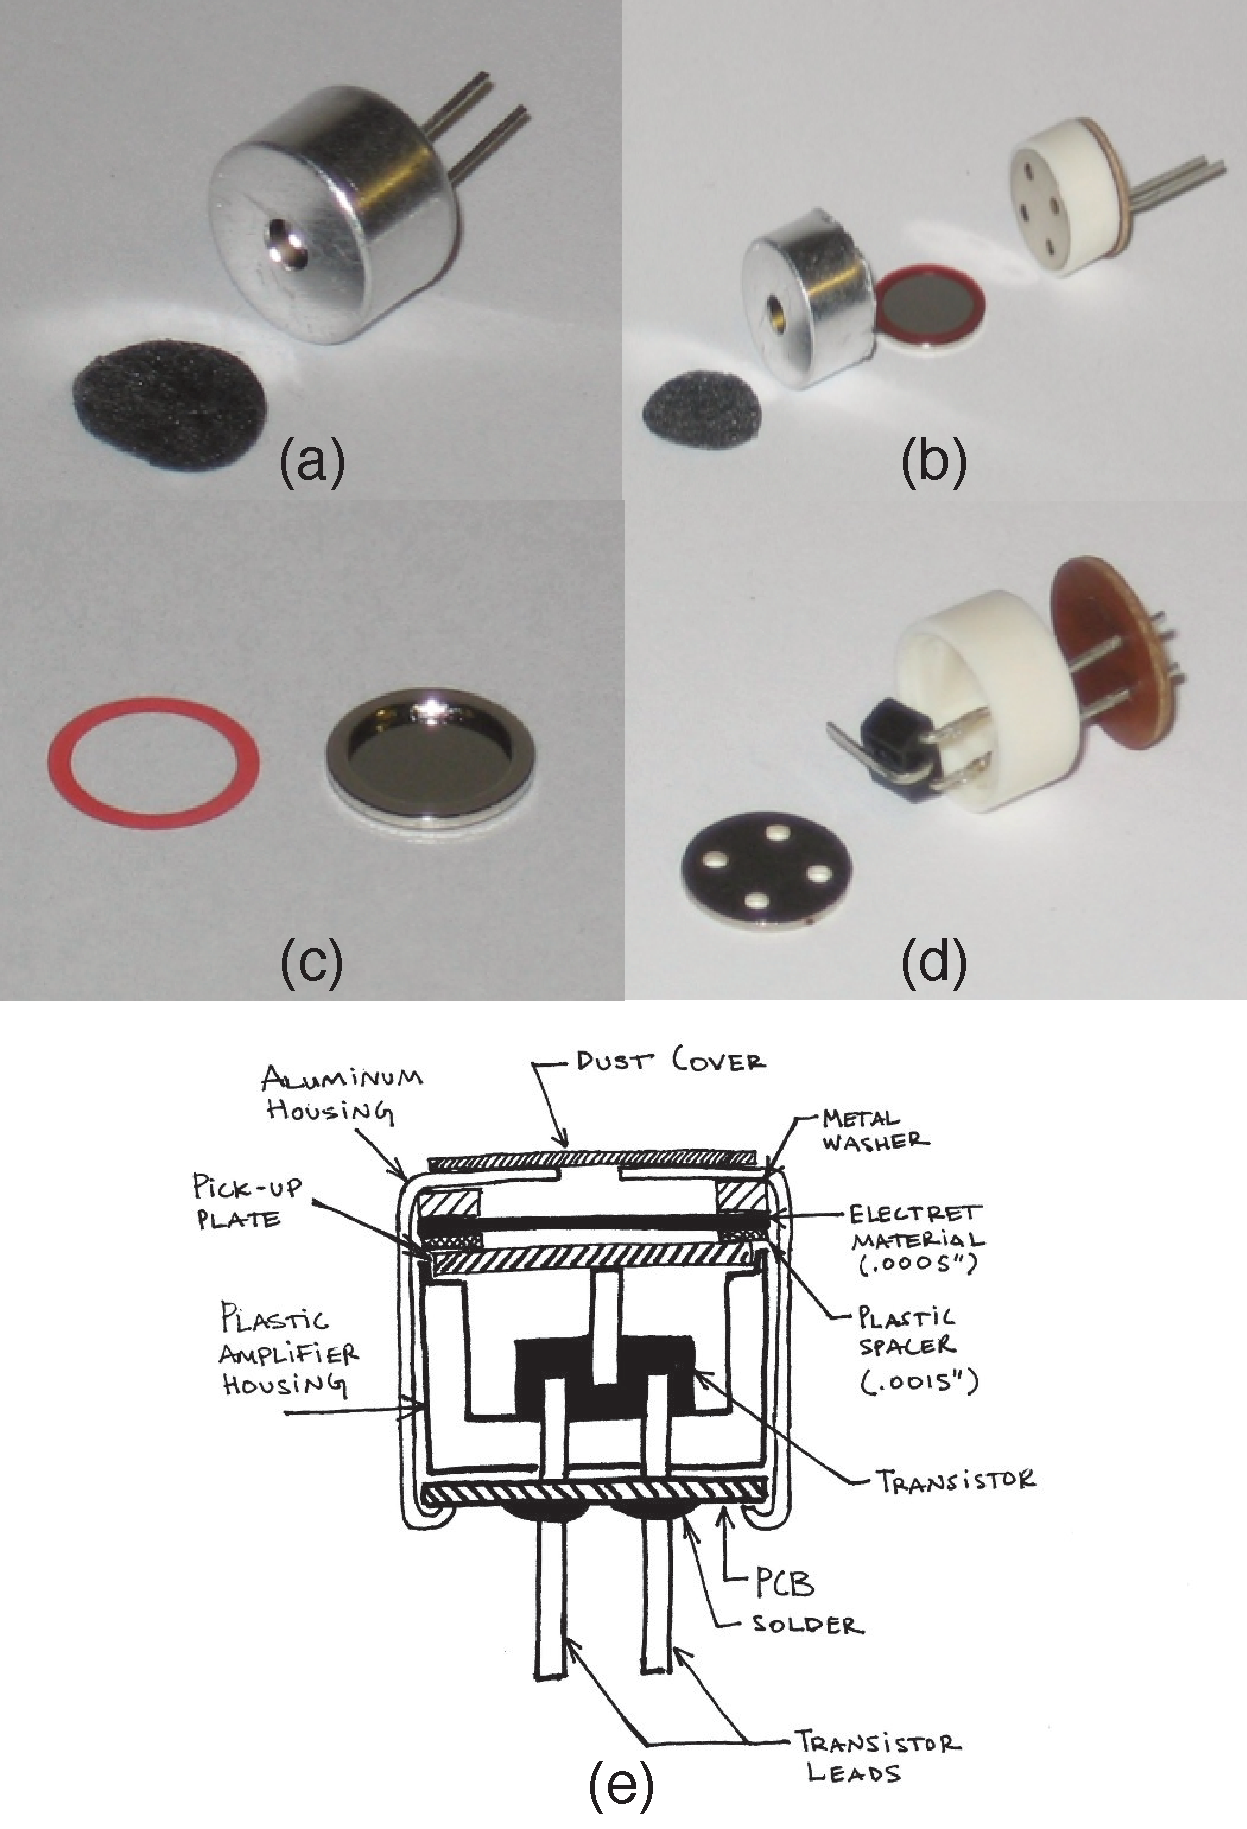
\includegraphics[width=0.6\textwidth,trim=0 0 0 0,clip=false]{electretmicpics.pdf}
\caption{Electret microphone anatomy. (a) With the dust cover removed, you can see the hole in the aluminum capsule, through which sound enters the mic. 
(b) At the next stage of deconstruction, you can see the electret diaphragm, which moves up and down in response to moving air.
(c) The red plastic spacer insulates the diaphragm and the metal washer it is mounted on from the amplifier pick-up plate (the plate with four holes in (d)). 
(d) The amplifier module consists of the pick-up plate, a plastic housing, a JFET transistor, and the PCB. 
The pick-up plate makes electrical contact with the bent gate lead of the JFET.
Images from www.openmusiclabs.com.}
\label{fig:3}
\end{center}
\end{figure}

\begin{figure}[!h]
\begin{center}
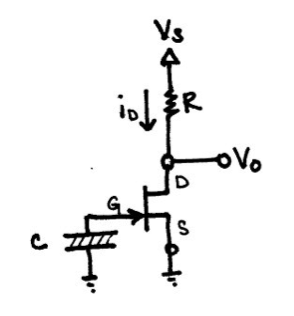
\includegraphics[width=0.4\textwidth,trim=0 0 0 0,clip=false]{images/insideelectretschematic.png}
\caption{Electrical schematic of electret insides (except for the resistor - that you will add on).
Image from www.openmusiclabs.com.}
\label{fig:4}
\end{center}
\end{figure}

\pagebreak

\item {\bf  Building the microphone circuit}\\
Build the circuit shown in Fig. \ref{fig:2} on a breadboard. 
Note which pin should be go to the output and which should go to ground as shown in Fig. \ref{fig:1}.\\
{\bf Question:} What function do you think the resistor between the 5 V source and the output serves? 

\begin{figure}[!h]
\begin{center}
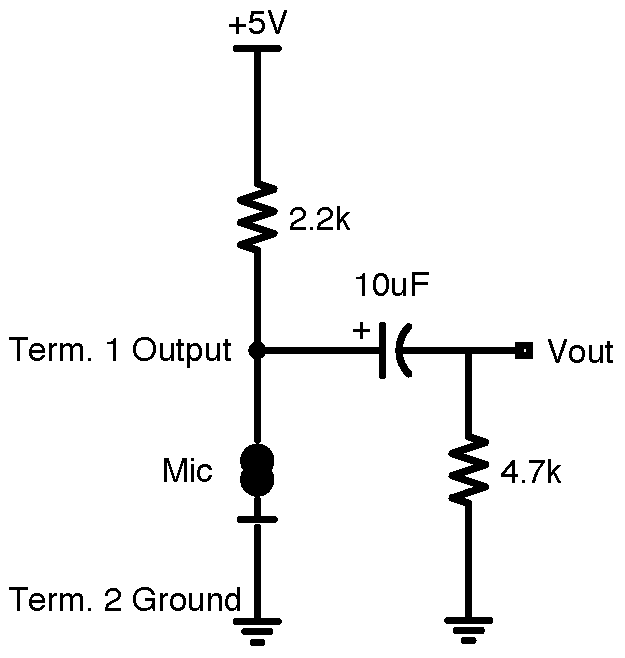
\includegraphics[width=0.35\textwidth,trim=0 0 0 0,clip=false]{circuitdiagram.pdf}
\caption{Microphone circuit to build.}
\label{fig:2}
\end{center}
\end{figure}

\begin{figure}[!h]
\begin{center}
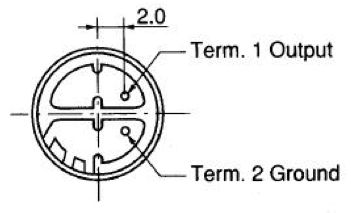
\includegraphics[width=0.25\textwidth,trim=0 0 0 0,clip=false]{electretpinout.png}
\caption{Electret microphone pinout diagram (the perspective is from underneath the microphone). 
The Output pin will connect to the resistor and electrolytic capacitor.}
\label{fig:1}
\end{center}
\end{figure}

\item {\bf Observing noise and measuring signals from the microphone using the oscilloscope}
\begin{enumerate} 
\item Plug in your scope leads to the oscilloscope. 
\item Move the scope leads close to an AC outlet (NOT IN IT THOUGH!!), or near fans or cables behind the computer. You should see 60 Hz and other noise. Does the noise change appreciably when you hold the leads straight, parallel and together, versus pulled apart? If so, why?
\item Connect the microphone circuit output and ground to the scope. What is the approximate RMS noise voltage you see on the scope (without anyone talking into the microphone, but with the 5 V DC power supply connected)?
\item Talk into the microphone at a comfortable level. What is the approximate RMS voltage you generate while talking? What, then, is your SNR?
\item Once you confirm that your circuit is working, show it to the TA and then transfer it to perfboard to make it more mechanically stable, 
using solder to make connections.
%take a few minutes to make it more mechanically stable by trimming down the resistor and capacitor leads, and wrapping signal and power wires around the power posts (or through the post holes if the posts are not there). Verify that your circuit works.
\end{enumerate}

\item {\bf Processing audio signals using LabView}
\begin{enumerate}
\item Connect the output and ground of your microphone circuit to the analog input channel 0 (\textbf{ACH0}) of your NI board (using a BNC cable with alligator clips, not oscilloscope leads). 
\item Modify your VI created earlier by changing the sampling rate to 10 kHz. Change the buffer size to store 1/10th of a second. 
Verify that you can see signals from your microphone and that your frequency display now shows appropriate values.
\item Zoom in on a very small time/voltage window of your signal (10 ms is good), so you're only looking at noise. 
Notice the quantization error. Can you estimate the voltage step size of the ADC (i.e., the voltage increment corresponding to the least significant bit)?
Compare this to the RMS noise voltage of the microphone that you measured on the oscilloscope -- is the DNR acceptable here? How many bits of noise do you have? 
Suppose you determined the quantization error was too high. What would you need to change?
\item Make sure the buffer size is 1/10th of a second. 
Pick the best singer in your team (best to determine this by a singing competition) and have that person try to hum a pure tone.  
Observe the time/frequency plots.  What is the range of frequencies that you can hum?  
How close are these to pure tones (i.e. single frequency sinusoids)?  
If youÕre musically inclined, try humming a scale and observing how the frequency spectrum changes.  
\item Add a numeric indicator on your GUI which displays the total RMS signal amplitude in volts.  
You may find the ``Amplitude and Level Measurements'' express VI handy.  
\item Add a numeric indicator which displays the fundamental frequency.  You may want to use the ``Tone Measurements'' express VI. 
\item Do you notice any differences between the spectrum of you and your partnerÕs voice?  
These should be particularly apparent if you have a male-female team.  
For the remainder of the lab, 
try to use the toolboxes available to you in Labview to develop an 
algorithm to distinguish two of the members in your group using the data in the frequency or time domain.  
The algorithm should output two Boolean values: one for each of you.  
These should light up LED indicators on your GUI.  
There are many approaches to this, so be creative.  Here are some ideas to get you started:
\begin{enumerate} 
\item Make a decision using the power and fundamental frequency that you calculate for (e) and (f), with appropriate thresholds for each.  If power is over a certain amount, assume that someone is talking.  
If the peak frequency is above/below a certain amount select one person or the other.  
Does it work better to identify people based on single vowels, or regular speech? Why?
\item If the frequency content of your voices occurs in distinct ranges, you could calculate the total power in those ranges and see if itÕs over a certain threshold.  This may be a little more robust than (i).
\item Record two waveforms of you and your partner saying the same thing.  Store these two waveforms in a local variable.  Then use a cross-correlation block to compare the sampled waveform with these saved waveforms.  If the cross-correlation is particularly high, consider it as a match.
\end{enumerate}
Another cool idea to think about: 
Notice on the frequency plots that your pitch shifts over time even when you try to hold it steady, unless you have a well trained voice. 
This is the motivation for autotuners used (excessively) in music today. 
What can you do to produce a spectrograph immune to this drift? 
Can you make a single-note autotuner in LabView?

\end{enumerate}

\noindent Parts List:\\[0.2em]
\begin{tabular}{|r|l|}
\hline
BNC Coax cable & 1 \\ \hline
Electret Microphone & 1 \\ \hline
Hookup wire & \\ \hline
2.2 k$\Omega$ Resistor & 1 \\ \hline
10 uF Electrolytic Cap & 1 \\ \hline
4.7 k$\Omega$ Resistor & 1 \\ \hline
BNC Coax Cable with Alligator Clips & 1 \\ \hline
Oscilloscope Leads & 1 \\ \hline
Breadboard & 1 \\ \hline
\end{tabular}

\end{enumerate}
\end{document} 